% ==========================================================================
%  Radio Telescope -- research poster template
%  48 in x 36 in landscape (4:3), Duke glass theme
%
%  Build with XeLaTeX (or LuaLaTeX) -- pdfLaTeX can't load the fonts:
%     latexmk -xelatex poster.tex
%  or by hand:
%     xelatex poster && bibtex poster && xelatex poster && xelatex poster
%  Overleaf: Menu -> Compiler -> XeLaTeX, and upload the fonts/ folder.
%
%  Folder layout
%     beamerthemedukeglass.sty   all styling lives here
%     fonts/                     Instrument Serif + EB Garamond (OFL)
%     figures/                   your images  (>= 150 dpi at printed size)
%     logos/                     duke.pdf / duke.png  (official mark)
%     poster.bib                 references
%
%  Every \posterfigure{file}{label} shows a labelled placeholder until
%  <file> exists -- drop the image in figures/ with that name and recompile.
%
%  Design notes (Duke MCL poster guide): text sparingly, generous white
%  space, read top-left to bottom-right column by column, 2-3 colours,
%  title >= 85 pt / authors >= 56 / headings >= 36 / body >= 24 / captions
%  >= 18. The theme already sets sizes above these minimums.
% ==========================================================================

\documentclass[final]{beamer}

\usepackage[size=custom, width=121.92, height=91.44, scale=1.0]{beamerposter}
\usetheme{dukeglass}
\usetikzlibrary{angles,quotes,arrows.meta}
\usepackage{graphicx}
\usepackage{booktabs}
\usepackage{amsmath}
\usepackage{siunitx}
\sisetup{separate-uncertainty=true, mode=text}

% numbered reference line (set compactly in the References box)
\newcommand{\refitem}[1]{{\color{dukeroyal}[#1]}\enspace}
% \cite{key} prints the matching number from the hand-typeset References box.
% Keep these in step with the \refitem numbers there and with poster.bib.
\newcommand{\refnumperley}{1}\newcommand{\refnummacgregor}{2}
\newcommand{\refnumtms}{3}\newcommand{\refnumnvss}{4}
\newcommand{\refnumalfalfa}{5}\newcommand{\refnumsimbad}{6}
\renewcommand{\cite}[1]{{\color{dukeroyal}[\csname refnum#1\endcsname]}}
\usepackage{pgfplots}
\pgfplotsset{compat=1.18}

% ====================
%  Columns: three equal columns, read left to right
% ====================
\newlength{\colgap}   \setlength{\colgap}{2.6cm}
\newlength{\colwidth}
\setlength{\colwidth}{(\paperwidth - 2\posteredge - 2\colgap)/3}
\newcommand{\outercolumn}{\begin{column}{\posteredge}\end{column}}
\newcommand{\gapcolumn}{\begin{column}{\colgap}\end{column}}

% \sidebyside{<left file>}{<right file>}: two images at a common height,
% scaled together so the pair (plus a 1 cm gap) exactly fills \linewidth.
\newsavebox{\sbsleft}\newsavebox{\sbsright}
\newlength{\sbsgap}\setlength{\sbsgap}{1cm}
\newlength{\sbsheight}
\newcommand{\sidebyside}[2]{%
  \sbox{\sbsleft}{\includegraphics[height=10cm]{#1}}%
  \sbox{\sbsright}{\includegraphics[height=10cm]{#2}}%
  \setlength{\sbsheight}{\dimexpr 10cm*\numexpr\dimexpr\linewidth-\sbsgap\relax/1024\relax/\numexpr\dimexpr\wd\sbsleft+\wd\sbsright\relax/1024\relax\relax}%
  \mbox{\includegraphics[height=\sbsheight]{#1}\hspace{\sbsgap}\includegraphics[height=\sbsheight]{#2}}}

% ====================
%  Title block
% ====================
\title{Duke Radio Telescope}

\author{Roshan Sundaram \quad\textperiodcentered\quad John Button \quad\textperiodcentered\quad Professor Michael Gehm}

\institute{Department of Electrical \& Computer Engineering, Duke University}

% ====================
%  Header logos  (left: institution, right: QR to project page)
% ====================
% Left title bubble: the white Duke logo on a transparent background.
% duke-white-trimmed.png is logos/duke-white.png with its empty margins cropped.
\logoleft{%
  \IfFileExists{logos/duke-white-trimmed.png}
    {
\includegraphics[width=\linewidth, height=7cm, keepaspectratio]{logos/duke-white-trimmed.png}}
    {
\includegraphics[width=\linewidth, height=7cm, keepaspectratio]{logos/duke-white.png}}}

% \logoright{\posterqr[7cm]{https://roshsun.com}}  % <- your project URL / duke.is link

% ====================
%  Footer
% ====================
\footercontent{%
  \href{mailto:roshan.sundaram@duke.edu}{roshan.sundaram@duke.edu}
  \hfill \hfill December 3, 2026
  % \hfill \href{https://roshsun.com}{roshsun.com}
  }

% ==========================================================================
\begin{document}
\begin{frame}[t]
  \begin{columns}[t, totalwidth=\paperwidth]

    \outercolumn

    % --------------------------------------------------------------------------
    %  Column 1 -- why and what
    % --------------------------------------------------------------------------
    \begin{column}{\colwidth}

      \begin{block}{Motivation}
        Radio astronomy is a practical means to understanding electromagnetic behavior and gaining hands-on experience with radio frequency (RF) hardware. We focused on neutral hydrogen (HI), which emits at 1420 MHz. We evaluated the feasibility of a radio telescope at Duke and simulated the performance of various configurations of receivers. We then studied the capabilities of a single antenna, acquired components, and verified them against their datasheets.

        %   % \begin{figure}
        %   %   \posterfigure[0.5]{figures/hero.jpg}{Hero image\\[0.2em]
        %   %     \footnotesize e.g.\ the dish, the receiver bench, or the sky target}
        %   %   \caption{[One-line caption.]}
        %   % \end{figure}
      \end{block}

      \begin{block}{Objectives}
        \textbf{Goal:} model an array of low-cost antennas across Duke's campus and deploy at scale.
        \begin{enumerate}
          \item \textbf{Build:} the 1\textsuperscript{st} iteration Duke Radio Telescope,
                and a radio astronomy community around it.
          \item \textbf{Simulate:} predict what the telescope should be able to see.
          \item \textbf{Test:} compare hardware performance to simulation results.
        \end{enumerate}
      \end{block}


      \begin{exampleblock}{Background}
        \setlength{\abovedisplayskip}{14pt}\setlength{\belowdisplayskip}{14pt}%
        \noindent\begin{minipage}[c]{0.58\linewidth}
          \textbf{Resolution.} A dish of diameter $D$ resolves
          $\theta_{\text{rad}}\approx\lambda/D \;\Rightarrow\; \theta_{\text{arcsec}}\approx 2\lambda_{\text{cm}}/D_{\text{km}}$.
          An interferometer replaces $D$ with the separation between antennas.

          \textbf{Baseline.} Each antenna pair is a baseline along $\hat{\mathbf{x}}$:
          $\mathbf{b}=|\mathbf{b}|\,\hat{\mathbf{x}}$, $u=|\mathbf{b}|/\lambda$. A source in direction
          $\mathbf{s}$ reaches one antenna later by the extra path $\mathbf{b}\cdot\mathbf{s}$
          (delay $\tau_g=\mathbf{b}\cdot\mathbf{s}/c$). Projecting $\mathbf{s}$ onto the baseline gives
          $\boldsymbol{l}=\hat{\mathbf{x}}\cdot\mathbf{s}=\sin\theta$; in 2-D,
          $\mathbf{b}\cdot\mathbf{s}/\lambda=u\boldsymbol{l}+v\boldsymbol{m}$.
        \end{minipage}\hfill
        \begin{minipage}[c]{0.45\linewidth}
          \includegraphics[width=\linewidth]{figures/extra_path_standalone-1.pdf}
        \end{minipage}

        \textbf{Fringe.} The delay is a phase that changes with sky position, so each baseline
        lays stripes $\lambda/|\mathbf{b}|$ apart across the sky:
        $F(\boldsymbol{l},\boldsymbol{m})=\cos 2\pi(u\boldsymbol{l}+v\boldsymbol{m})$.

        \textbf{Correlation.} The correlator multiplies the two voltages and time-averages:
        \[
          \langle V_1V_2\rangle=\tfrac{E^2}{2}\Bigl[\cos\omega\tau_g+
            \underbrace{\langle\cos(2\omega t-\omega\tau_g)\rangle}_{\to\,0}\Bigr]
          =P\cos\frac{2\pi\,\mathbf{b}\cdot\mathbf{s}}{\lambda}
        \]
        A point source of power $P$ at $(\boldsymbol{l}_0,\boldsymbol{m}_0)$ gives $P$ times the
        fringe there, $R=P\,F(\boldsymbol{l}_0,\boldsymbol{m}_0)$; an extended sky of brightness
        $I$ gives $R=\iint I\,F\,d\boldsymbol{l}\,d\boldsymbol{m}$.

        \textbf{Visibility.} A cosine fringe $R_C$ is even and misses odd structure, so a
        $90^\circ$ shift in one path adds a sine fringe $R_S$. Combined, they give a 2-D
        Fourier transform of the sky:
        \begin{gather*}
          V(u,v)=R_C-jR_S=\iint I(\boldsymbol{l},\boldsymbol{m})\,
          e^{-2\pi j(u\boldsymbol{l}+v\boldsymbol{m})}\,d\boldsymbol{l}\,d\boldsymbol{m}
        \end{gather*}

        \textbf{Image.} The array measures $V$ only at its baselines: the sampling function
        $S$ is 1 at each sampled $(u,v)$ and 0 elsewhere. Inverse-transforming, by the
        convolution theorem:
        \[
          I_{\text{obs}}=\mathcal{F}^{-1}\{S\cdot V\}
          =\underbrace{\mathcal{F}^{-1}\{S\}}_{B}\ast\underbrace{\mathcal{F}^{-1}\{V\}}_{I},
          \qquad B(\boldsymbol{l},\boldsymbol{m})=\sum_k\cos 2\pi(u_k\boldsymbol{l}+v_k\boldsymbol{m})
        \]
        The PSF $B$ is the sum of every baseline's fringe; the observed image is the
        true sky blurred by it.
      \end{exampleblock}

      \begin{tcolorbox}[section, top=0.4cm, bottom=0pt]
        \tiny\setlength{\parskip}{0pt}\setlength{\parindent}{0pt}
        {\large\displayfont\color{dukenavy}References}\par\vspace{0.1cm}
        \refitem{1}R.~Perley, \emph{Fundamentals of Radio Interferometry 1: The Basics}, CSIRO Radio School, Narrabri, NSW, 2023.\par
        \refitem{2}M.~MacGregor, \emph{Introduction to Radio Interferometry}, lecture slides, Carnegie DTM, 2018.\par
        \refitem{3}A.~R.~Thompson, J.~M.~Moran, G.~W.~Swenson~Jr., \emph{Interferometry and Synthesis in Radio Astronomy}, 3rd~ed., Springer, 2017.\par
        \refitem{4}J.~J.~Condon \emph{et al.}, ``The NRAO VLA Sky Survey,'' \emph{AJ} 115, 1693 (1998).\par
        \refitem{5}M.~P.~Haynes \emph{et al.}, ``The ALFALFA extragalactic H\,I source catalog,'' \emph{ApJ} 861, 49 (2018).\par
        \refitem{6}M.~Wenger \emph{et al.}, ``The SIMBAD astronomical database,'' \emph{A\&AS} 143, 9 (2000).\par
      \end{tcolorbox}
    \end{column}

    \gapcolumn

    % --------------------------------------------------------------------------
    %  Column 2 -- how
    % --------------------------------------------------------------------------
    \begin{column}{\colwidth}

      \begin{block}{Baseline Simulation}
        In the Spring, we simulated the performance of an array with 16 anetnnas placed on various rooftops on campus. Each pair of receivers creates a baseline, of which there are 120. Each baseline gives a point and its mirror, or 240 points in the $uv$ plane in Fourier space. The PSF measures how the array responds to an ideal point source. With 16 antennas, the PSF has a sharp central peak with sidelobes that blur the simulated image.
        \begin{figure}
          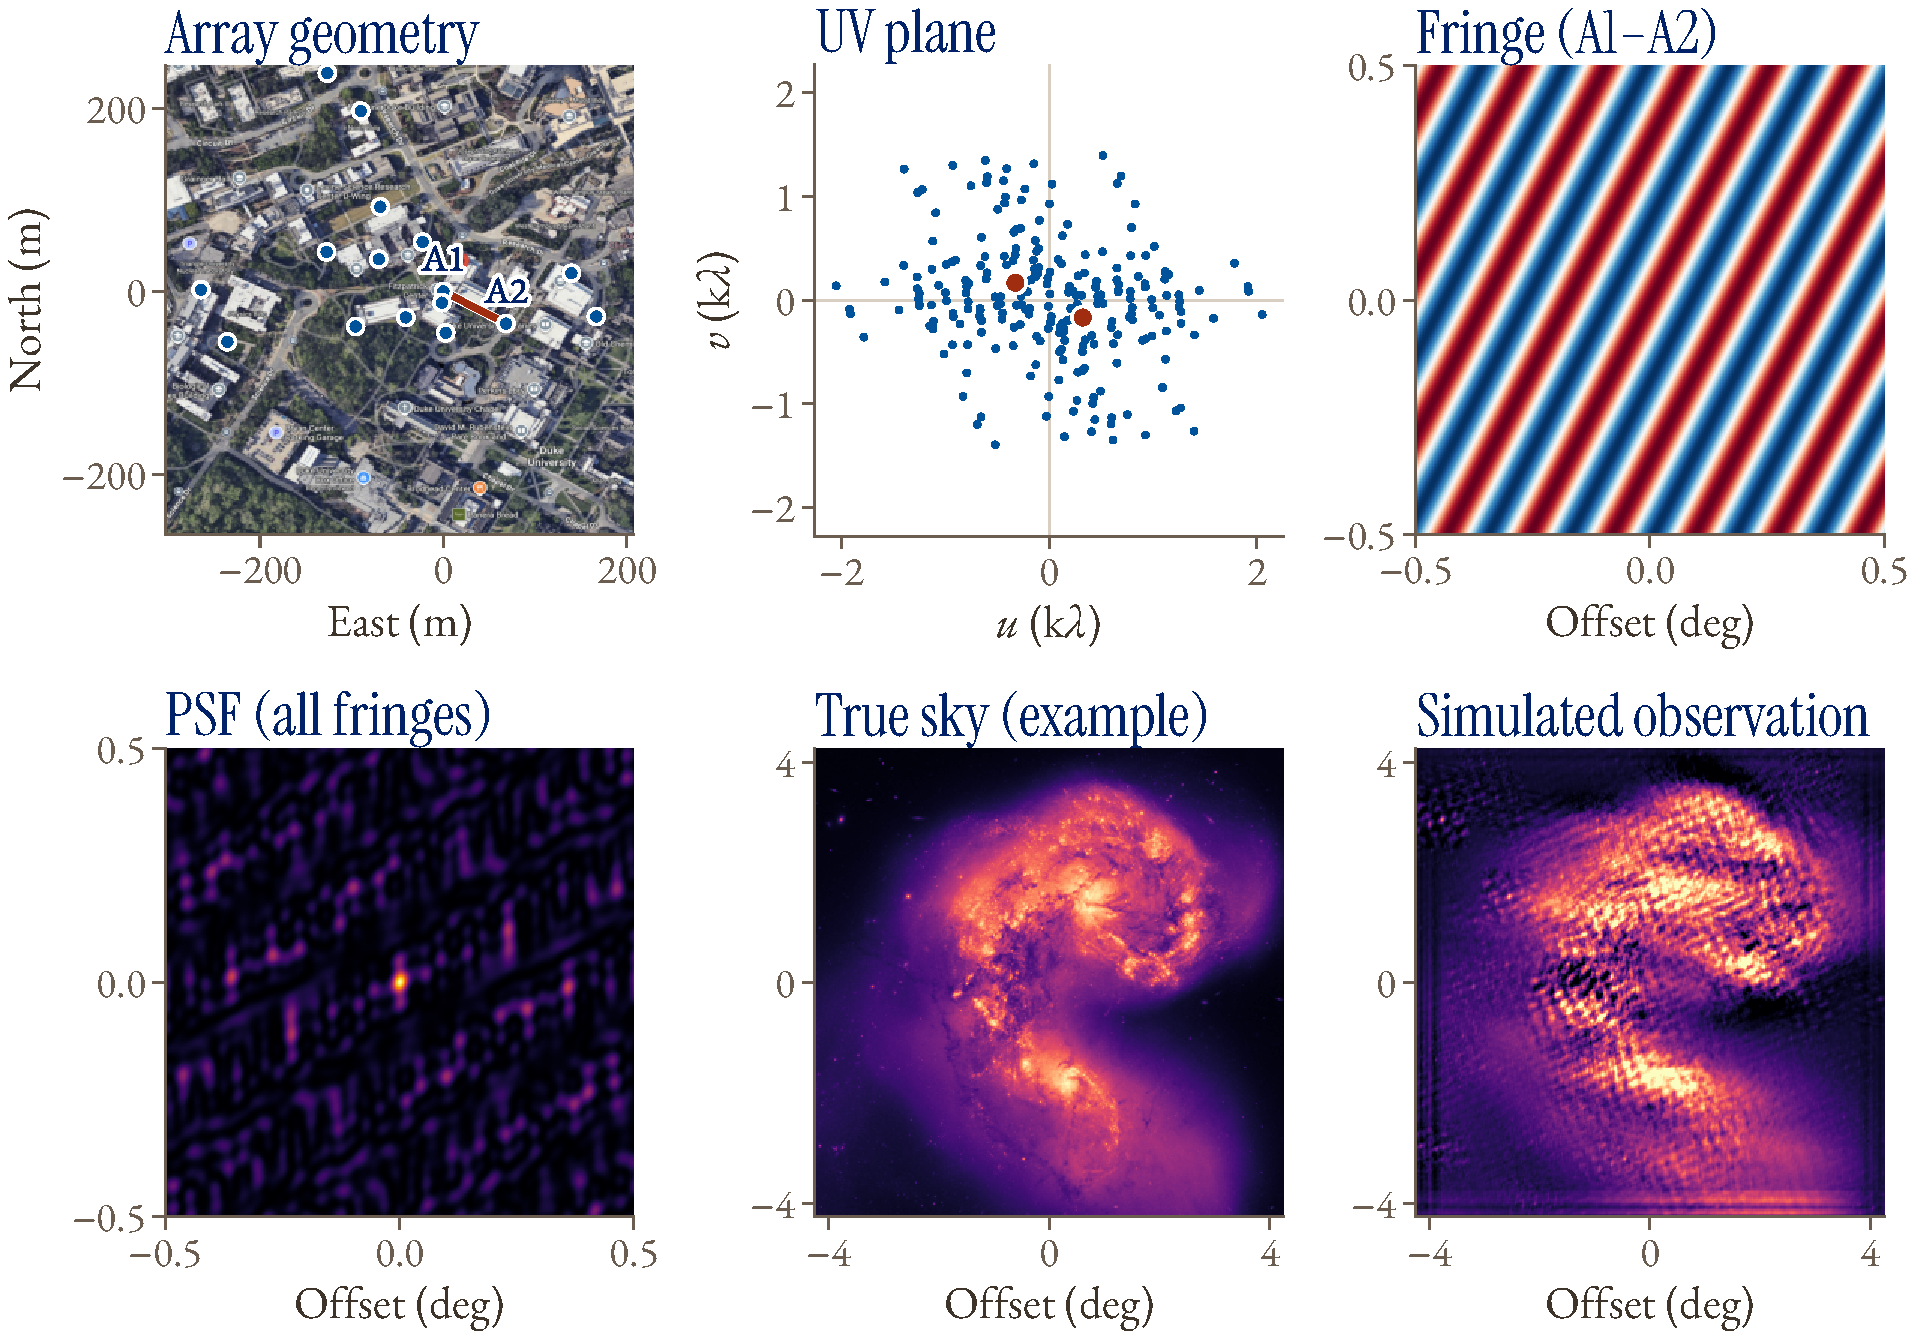
\includegraphics[width=\linewidth]{figures/array_simulation.pdf}
          \caption{Selected antenna locations (approximate) on Duke campus transformed into Fourier space. Each baseline creates a fringe. All fringes sum to create the PSF, which blurs an example celestial body into the simulated observation. Sky: Antennae Galaxies, ESA/Hubble \& NASA (potw1345a). }
        \end{figure}
      \end{block}

      \begin{block}{Beam Path \& Observable Bodies}
        This semester, we studied the capabilities of a single antenna: with only one receiver, what celestial bodies could we potentially observe? We built a program that would take in a location, antenna parameters, and receiver parameters to generate a beamwidth of the telescope, swept over a track in the sky as time progressed. We also identified potential sources in an astronomical database that would land in our telescope's ideal beam track.

        \begin{figure}
          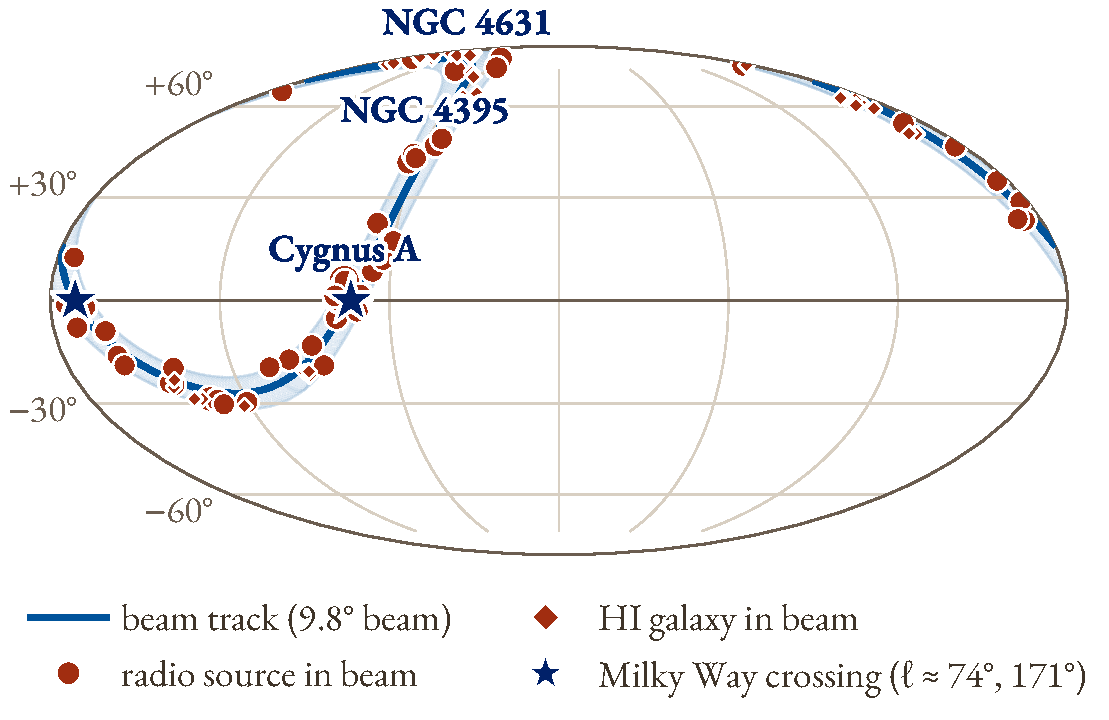
\includegraphics[width=0.6\linewidth]{figures/sky_galactic.pdf}
          \caption{Expected object visibility simulation with a single dish on Fitzpatrick roof. Sources from NVSS \cite{nvss} and ALFALFA \cite{alfalfa}, named via SIMBAD \cite{simbad}.}
        \end{figure}
      \end{block}




    \end{column}

    \gapcolumn

    % --------------------------------------------------------------------------
    %  Column 3 -- what we found, what's next
    % --------------------------------------------------------------------------
    \begin{column}{\colwidth}

      \begin{block}{Receiver Chain Testing}
        We developed a simple RF chain from the low-cost, hobbyist components below. The antenna was outside this semester's scope, so we focused on the receiver: the path from the antenna's feed to the measurement device. The weak signal from space is amplified, then filtered.
        \begin{center}
          % Receiver chain: antenna -> feed cable -> LNA -> filter -> SDR/VNA
% Drawn at real size for one poster column (~37 cm); use \input, not \resizebox.
% Needs: calc (loaded by the theme).
\begin{tikzpicture}[
    >=stealth,
    stage/.style={draw=dukenavy, fill=white, line width=2pt,
                  minimum height=3.2cm, minimum width=6.2cm,
                  align=center, font=\footnotesize, text=ink, inner sep=0.2cm},
    untested/.style={dash pattern=on 10pt off 7pt},
    link/.style={->, dukeroyal, line width=2.5pt, shorten >=2pt, shorten <=2pt},
    note/.style={font=\scriptsize\itshape, text=inksoft, align=center},
  ]
  \def\gap{1.5}  % arrow length between stages (cm)

  % ---- antenna (not yet tested in hardware) ----------------------
  \node[stage, untested, minimum width=3.6cm] (ant) at (0,0) {};
  \begin{scope}[shift={(ant.center)}, dukenavy, line width=2.5pt, line cap=round]
    \draw (0,-1.1) -- (0,0.35);            % mast
    \draw (0,0.35) -- (-0.9,1.15);         % V elements
    \draw (0,0.35) -- (0.9,1.15);
    \draw (-0.55,-1.1) -- (0.55,-1.1);     % ground
  \end{scope}


  % ---- the rest of the chain -------------------------------------
  \node[stage, anchor=west] (cab) at ($(ant.east)+(\gap,0)$) {Feed\\Cable};
  \node[stage, anchor=west] (lna) at ($(cab.east)+(\gap,0)$) {Low-Noise\\Amplifier};
  \node[stage, anchor=west] (fil) at ($(lna.east)+(\gap,0)$) {Band Pass\\Filter};
  \node[stage, anchor=west, fill=dukenavy, text=white] (sdr)
    at ($(fil.east)+(\gap,0)$) {Software-Defined\\Radio};

  % ---- part numbers under each stage ------------------------------
  \foreach \n/\t in {cab/{$50 \Omega$ Coaxial Cable},
                      lna/{Mini-Circuits\\ZX60-P162LN+},
                      fil/{GPIO Labs\\\SI{1420}{\mega\hertz} BPF},
                      sdr/{RTL-SDR v3}}
    \node[note, anchor=north] at ($(\n.south)+(0,-0.25)$) {\t};

  \foreach \a/\b in {ant/cab, cab/lna, lna/fil, fil/sdr}
    \draw[link] (\a.east) -- (\b.west);
\end{tikzpicture}

        \end{center}

        We wrote a program that simulated overall system gain and noise temperature from datasheet values of the selected components, and used it to order the chain above.
        To measure each part, we calibrated a vector network analyzer (VNA) and swept \SIrange{1220}{1620}{\mega\hertz}, centered on \SI{1420}{\mega\hertz}, validating each component against its datasheet. \SI{20}{\decibel} and \SI{30}{\decibel} attenuators protected the NanoVNA while we measured the LNA.
        \begin{center}
          \small\setlength{\tabcolsep}{16pt}\renewcommand{\arraystretch}{1.1}
          \begin{tabular}{l l r r}
            \toprule
            \textbf{Part} & \textbf{Measurement} & \textbf{Expected} & \textbf{Measured} \\
            \midrule
            \SI{20}{\decibel} Attenuator & Attenuation & \SI{20}{\decibel} & \SI{20.2}{\decibel} \\
            \SI{30}{\decibel} Attenuator & Attenuation & \SI{30}{\decibel} & \SI{30.1}{\decibel} \\
            Filter & In-band insertion loss & \SI{3}{\decibel} & \SI{2.56}{\decibel} \\
            Filter & \SI{-3}{\decibel} passband & \SIrange{1395}{1445}{\mega\hertz}
                   & \SIrange{1349}{1482}{\mega\hertz} \\
            LNA & Gain & \SI[retain-explicit-plus]{+19.81}{\decibel}
                @ \SI{1400}{\mega\hertz} & \SI[retain-explicit-plus]{+19.91}{\decibel} \\
            \bottomrule
          \end{tabular}
        \end{center}

        \begin{figure}
          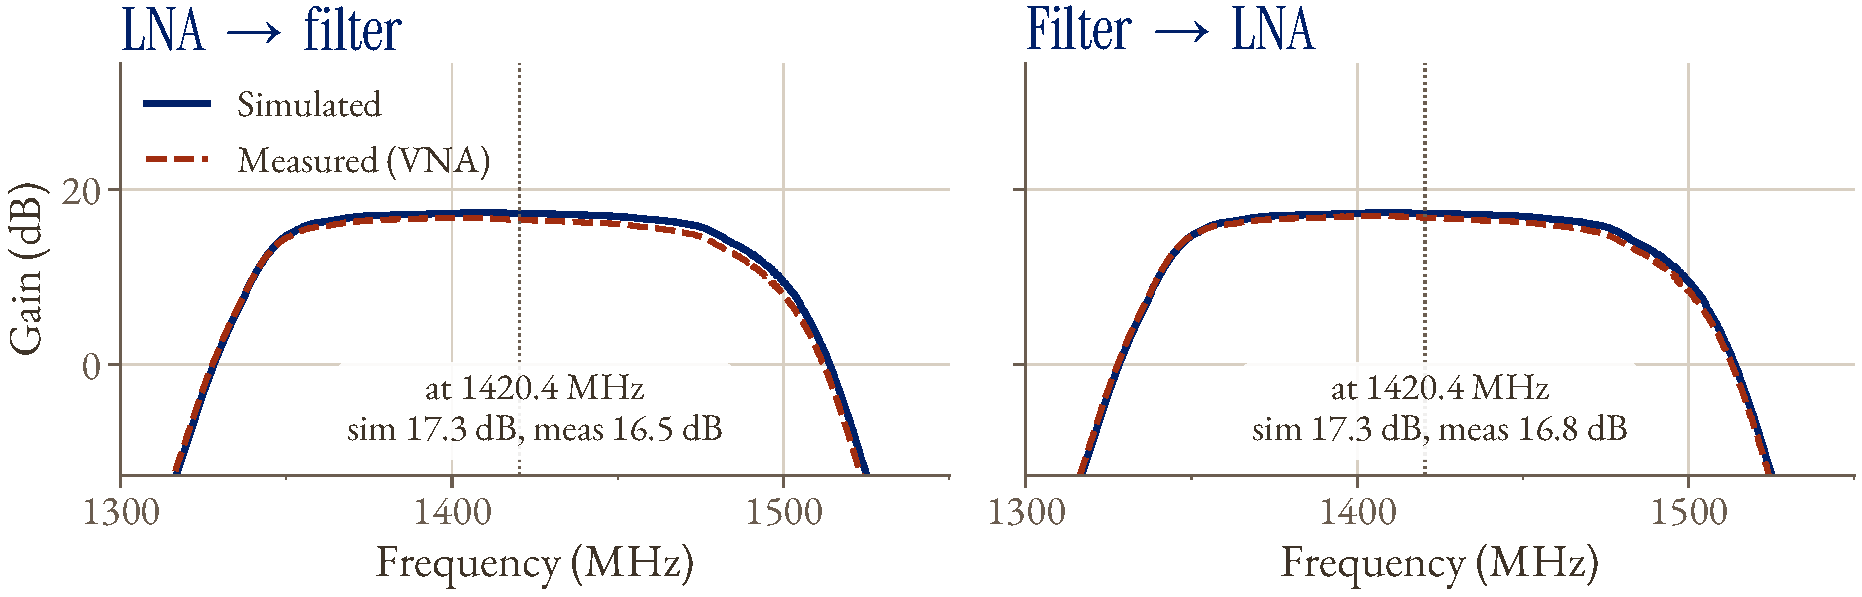
\includegraphics[width=0.85\linewidth]{figures/hardware_response.pdf}
          \caption{LNA + filter chain in both orders: simulated vs.\ measured, within \SI{0.8}{\decibel} at \SI{1420}{\mega\hertz}.}
        \end{figure}

        From our testing, we found that the current components are suitable for the first iteration of our RF chain. Of all components, the current filter deviated most from advertised specifications, especially regarding the pass band. A wider pass band admits more terrestrial noise around \SI{1420}{\mega\hertz}. We may purchase a filter with a narrower pass band if we deem this model to be insufficiently capable.
      \end{block}


      \begin{block}{Next Steps}
        \begin{enumerate}
          \item Buy the feed coax, then simulate and measure it as part of the chain.
          \item Simulate and fabricate the antenna, then measure it with the VNA.
          \item Integrate components and deploy at a suitable rooftop location on campus.
          \item Build data-collection and processing software with Raspberry Pi and RTL-SDR. 
        \end{enumerate}
      \end{block}

      \begin{block}{Acknowledgements}
        I would like to thank Professor Michael Gehm for his continued support on this project and for getting me interested in RF systems in ECE270!
      \end{block}

    \end{column}

    \outercolumn

  \end{columns}
\end{frame}
\end{document}
